柔軟な膜やケーブルで構成される宇宙構造は軽量・高収納率の展開構造として,薄型アンテナ,薄膜太陽電池アレー,ソーラーセイル,サンシールド,オカルタなど多様な宇宙利用が期待されている.近年,薄膜化が進むアンテナや太陽電池セルなど,各種薄型デバイスを膜構造上に貼付しながら,膜面構造を高収納率に収納し,高い信頼性で軌道上での展開を実現する構造様式(以降これを「多機能展開膜構造」と呼称する)の実証は特にいまだ希少である.デオービットを目的とした膜の展開実証は為されてきている一方で,薄膜デバイス搭載膜の宇宙実証については,2010年の小型ソーラー電力セイル実証機IKAROSおよび2017年の国際宇宙ステーション上でのRoll-Out Solar Array (ROSA)等の数例しかない.したがって開発コストが比較的安価であるCubeSatを用いて多機能展開膜の宇宙実証を行うことは意義が高い.また,CubeSatを用いて展開膜の展開挙動の動画撮影などを実施することが考えられるが,超小型衛星には通信レートの低さの課題がある.2012年にISSより放出された福岡工業大学の1U CubeSat FITSAT-1(にわか)は,アマチュア5.8GHz帯での115kbpsの通信に成功しており\cite{Tanak15acta},本技術の活用・発展が望まれる.
\begin{figure}[H]
	\centering
	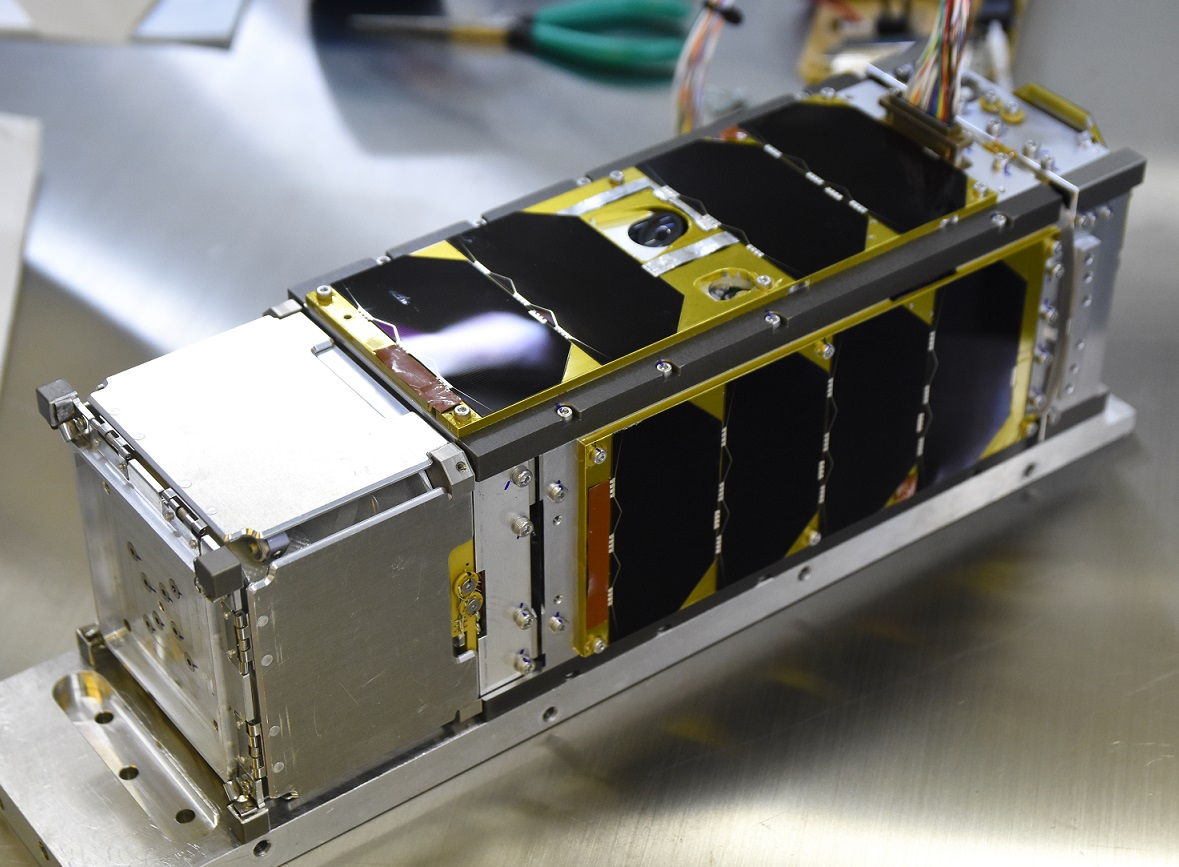
\includegraphics[width=0.7\linewidth]{01/fig/1-1-1.jpg}
	\caption{OrigamiSat-1フライトモデル}
	\label{fig1-1-1}
\end{figure}
\begin{figure}[H]
	\centering
	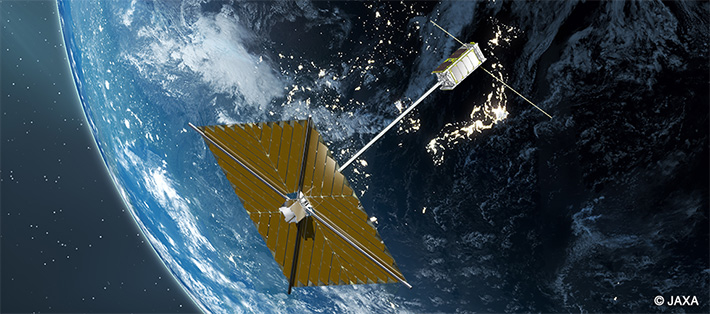
\includegraphics[width=1\linewidth]{01/fig/1-1-2.jpg}
	\caption{OrigamiSat-1軌道上での展開イメージ}
	\label{fig1-1-2}
\end{figure}

上記背景から,我々は3U CubeSat「OrigamiSat-1」を開発した.宇宙実証衛星を開発・運用するという活動を通して,大学が持つ技術シーズを実際の宇宙機器へ実装し,さらに開拓精神を持つ若手人材を育成する「宇宙展開構造物 研究開発拠点」を醸成することを目指す.OrigamiSat-1は以下の3つの主要ミッションを持つ.第一に,太陽発電アレーや平面アンテナを薄膜上で実現しうる,大幅な構造の軽量化・高収納率化を可能にするブーム・膜複合構造(著者らが提案)による「多機能展開膜構造」を宇宙実証する(多機能膜展開ミッション).第二に,3Uキューブサット上で各種展開構造物の宇宙実験を可能にし,今後も継続的に宇宙実証を活用した技術開発を行っていくための「実験プラットフォーム」を構築し,その宇宙実証を行う.OrigamiSat-1の3Uのうち,実験プラットフォーム部分が2Uサイズ,供試体が1Uサイズとする(宇宙実証プラットフォーム開発ミッション).第三に,5.8GHz帯でのアマチュア無線衛星通信技術を確立し,同周波数帯の普及に貢献する(アマチュア無線ミッション).
著者らは2015年1月から衛星の概念設計を開始し,(i) 多機能展開膜,(ii) 膜計測実験プラットフォームの2つの主要コンポーネントを新規に開発し,(iii) 5.8GHz通信系を実装し,また (iv) 上記3つのミッション系に対応するバス系を開発しシステムの統合を実施した.衛星は2018年11月にJAXAイプシロンロケット4号機へ引き渡され,2019年1月18日に高度500kmの軌道へ打ち上げられた.打ち上げ後,衛星からの信号を受信し,さらに地上局からのコマンドアップリンクによる衛星状態の取得を実施した.しかし,ミッションを開始する直前の,打ち上げから6日半が経過した時点で,地上局運用中に衛星からの信号が途絶える不具合が発生し,本報告書執筆時点で衛星との通信が復帰していない状態にある.


本報告書を次の3つの目的で執筆する.第一に,新規性の高い2種のミッション部の設計と,それらを3U CubeSatへ統合するためのバス部およびシステムの設計について記すことで,OrigamiSat-1が実装したCubeSat設計の知見を共有する.第二に,OrigamiSat-1の打ち上げ後からの発生事象を記すとともに,初歩的な不具合解析を示すことで,衛星バス部が直面している状況を共有し議論・学びの糧とする.第三に,OrigamiSat-1の開発過程を振り返り,その中で特徴的な失敗のエピソードを記す.これにより,教科書などに示されている衛星開発のデザインパターンを補間しうる,CubeSat開発のアンチパターンを抽出・体系化していく議論を喚起する.


